\Chapter{A szakdolgozat koncepciója}

A feladat fő problémája a háromszögek metszéspontjának kiszámítása a térben. Ez sajnos nem egy egyszerű feladat. Programozás, illetve erőforrásigény terén sem elhanyagolható.

A valóságban az emberi gondolkodásnak egyszerűnek tűnhet eldönteni, hogy két háromszög metszi-e egymást, vagy sem. Programozás, illetve matematika részéről viszont sokkal nehezebb. Rengeteg számítást kell végeznünk ahhoz, hogy megbizonyosodjunk a háromszögek metszéséről.

\Section{Irodalomkutatás}
A metszéspontok számításhoz legmegfelelőbbnek \href{https://www.geometrictools.com/Documentation/DynamicCollisionDetection.pdf}{David Eberly 1999-es kutatását}, azon belül a 4.1 Separation of Triangles\cite{triangles} szekciót találtam. A dokumentáció tökéletesen elmagyarázza a matematikai képletek elemeit, azok használatát, lépéseit. Ezek mind táblázatba szedve találhatóak. A pontos magyarázat a \ref{chap:utkozesek}. fejezetben található. Emellett rengeteg különböző módszer található az interneten térbeli modellek ütközésének vizsgálatához.\\
\newpage
\subsection{Négyzetes elválasztás (Quadratic Separation)}
\label{chap:quad}
A négyzetes elválasztás módszere egy olyan algoritmus, amelyet számítógépes játékok, illetve számítógépi grafikában közkedvelten használnak ütközések vizsgálatára.
A módszer segítségével meghatározhatjuk, hogy két vagy több modell metszi-e egymást vagy sem.
Az ötlet lényege, hogy minden modellt egy kocka alakú "dobozokkal" vesszük körbe, amelyet a legkisebb négyszögű terület alapján határozzuk meg. Ekkor az ütközést csak akkor kell ellenőrizni, ha a meghatározott "dobozok" metszik egymást.\\
Lépései:
\begin{itemize}
\item Minden modellhez rendelünk egy "dobozt", amely a legkisebb területen határozza meg a modellt. Ez a "doboz" könnyen meghatározható 2 ponttal a térben. A modellekhez társított területet a \ref{fig:con_1} ábrán láthatjuk.

\item Ellenőrizzük a "dobozokat", hogy metszi-e egymást vagy sem.

\item Ha két vagy több "doboz" metszik egymást, akkor kerül sor a pontos ütközésvizsgálatra (jelen szakdolgozat alapján ez háromszögek metszéspontjának számítása).
\end{itemize}
Az előnye a módszernek, hogy a bonyolult modelleket leírhatjuk először egyszerű geomatriai alakzattal, így az ütközésvizsgálat ideje nagyban csökken. Hátránya, hogy az algoritmus csak közelíti az eredményt, ezért fontos egyéb algoritmusokat alkalmazni a pontos ütközésvizsgálathoz.

\begin{figure}[h]
	\centering
	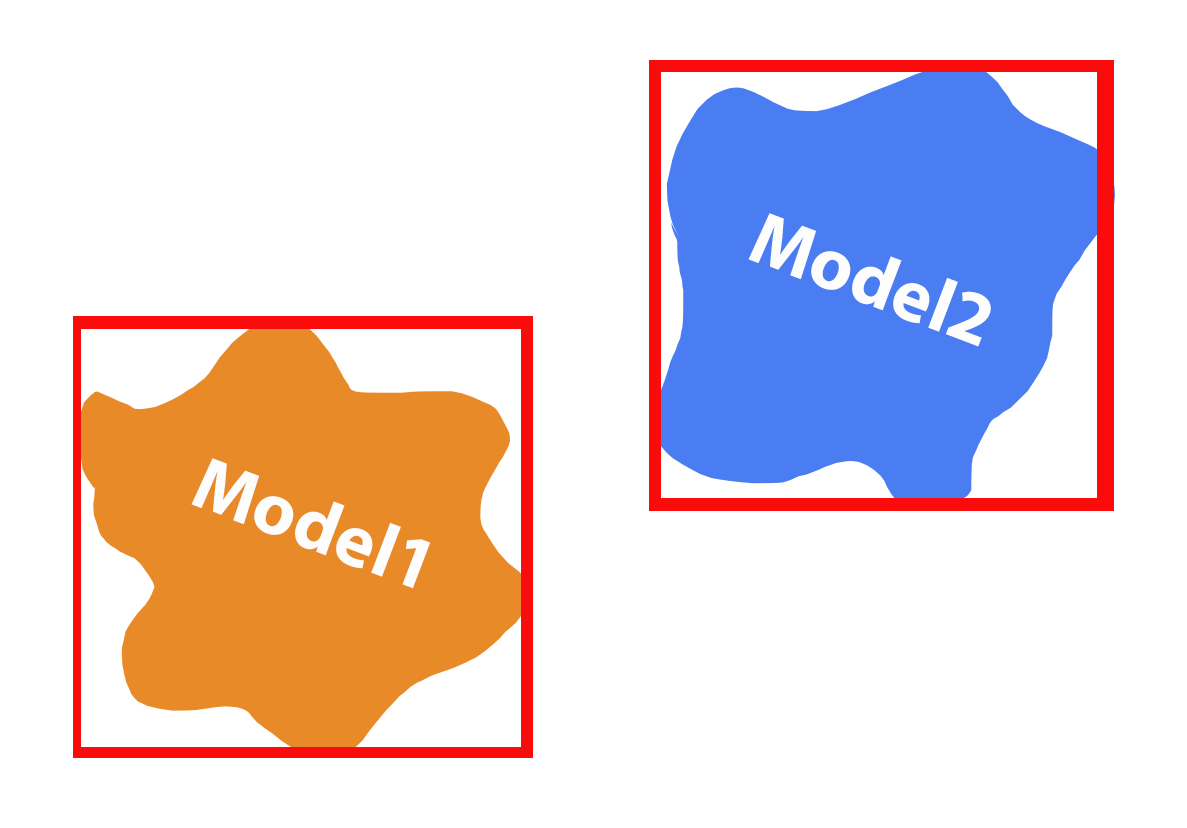
\includegraphics[width=13truecm, height=7.5truecm]{images/con1.png}
	\caption{Doboz rendelése modellekhez síkban ábrázolva}
	\label{fig:con_1}
\end{figure}


\newpage
\subsection{Voxel-alapú ütközésvizsgálat}
A voxel-alapú módszer egy hatékony módszer, amely a háromdimenziós teret felosztja kisebb részekre, téglalap alakú részekre. Ezeket a részeket voxelek-nek nevezzük.
Ezekkel a voxelekkel közelítjük a modelleket.
\\
Lépései:
\begin{itemize}
\item Voxel rácsot hozunk létre. Ezzel a ráccsal osztjuk fel a teret kisebb voxelekre. Ezt a módszert használhatjuk bármilyen dimenzióban.

\item A modelleket voxelekkel közelítjük, amelyek a voxel rácsban helyezkednek el. A pontosság módosítható a voxelek mérete alapján. Minden voxelt megjelöljük az alapján, hogy tartalmaz-e modellt vagy sem. A \ref{fig:con_3} ábra jól szemlélteti a modelleket körülvevő aktív voxel cellákat.

\item Ütközések vizsgálatához azt ellenőrizzük, hogy a két modellt tartalmazó voxel metszi-e egymást vagy sem. Ha egy aktív voxel metszi a másik aktív voxelt, akkor a modellek ütközhetnek egymással. Ezután szükséges egyéb ütközésvizsgálat a pontosításhoz.
\end{itemize}
Előnye a módszernek, hogy a használata egyszerű, a pontosság könnyen módosítható. Nagyobb tér esetén hatékony megoldás lehet. Az ütközésvizsgálat csak az aktív voxelek esetén történik meg, így elkerülhetőek a fölösleges számítások. Hátránya, hogy nehéz pontosan meghatározni a voxel rács méretét. Túl nagy méret esetén az ütközésvizsgálat nem lesz elég pontos, kis méret esetén a számítások költségesek lehetnek.
\begin{figure}[h]
	\centering
	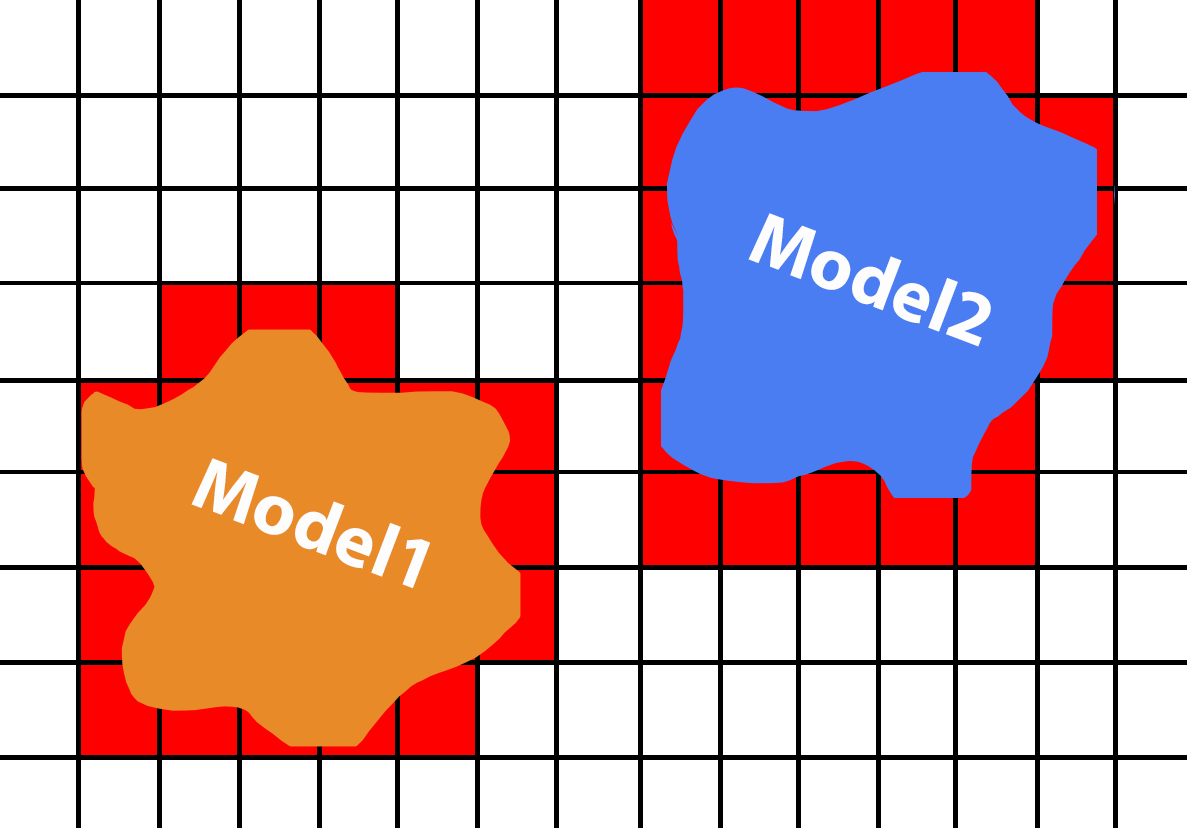
\includegraphics[width=13truecm, height=7.5truecm]{images/con3.png}
	\caption{A tér felbontása voxelekre a síkban}
	\label{fig:con_3}
\end{figure}

\newpage
\subsection{Egyenletek alkalmazása}
Az egyenletek alkalmazásának alapötlete, hogy matematikai egyenletek segítségével határozza meg a modellek mozgását, illetve ütközéseinek érzékelését.
\\
Lépései:
\begin{itemize}
\item Felállítunk egy matematikai modellt, amely leírja a modellek mozgását.

\item Definiáljuk az ütközések vizsgálatához szükséges szabályokat, feltételeket. Ezek a feltételek lehetnek egyszerűbbek, vagy komplexebbek, például távolságok, sebességek, fizikai tulajdonságok, formák, méretek.

\item A meghatározott modell és a feltételek alapján ellenőrizzük az ütközésvizsgálatot.\

\item Gyakran szükség van az egyenletek alkalmazására numerikus módszerekre, például differenciálegyenletek megoldása esetén.
\end{itemize}
Előnye a módszernek, hogy pontos fizikai szimulációkat érzékelhetünk. Hátránya, hogy sok esetben magas a számítási igénye, ezért nem alkalmas valós idejű szimulációkra, illetve magas modellszám esetén sem előnyös.